\chapter{Definición del problema}

\section{Contexto}

Actualmente, las aeronaves no tripuladas son utilizadas para actividades recreativas tanto como comerciales en la industria. Por nombrar algunas aplicaciones estas pueden ser agricultura donde se requiere monitorear cultivos, topografía para creación de mapas y planificación, búsqueda y rescate donde las aeronaves pueden abarcar un gran área mientras transmiten imágen en alta resolución, o para la fotografía en general. En \cref{fig:disco} se puede observar una aeronave tipo ala delta llamada ``Parrot Disco'' caracterizada por su capacidad de grabar video en alta resolución y ofrecer visión en primera persona, su controlador se puede programar con el software ArduPilot donde en su documentación se ofrecen instrucciones para ello \cite{disco2}.

\begin{figure}[h]
    \centering
    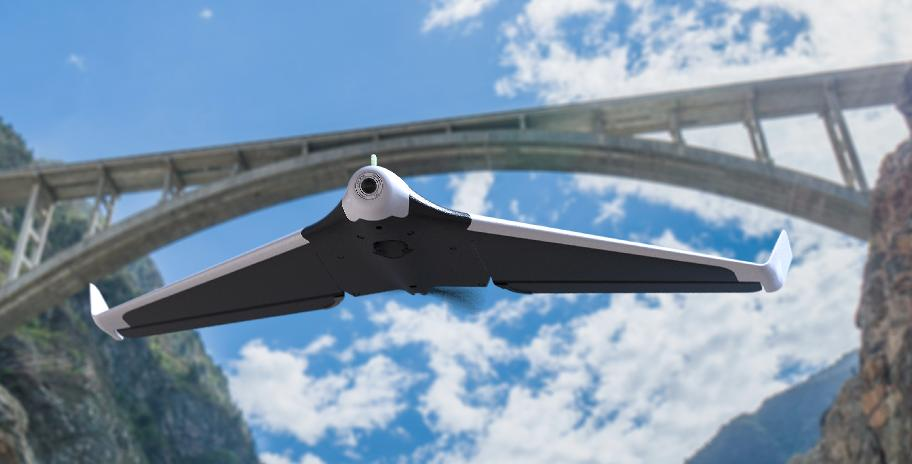
\includegraphics[width=0.6\textwidth]{disco-flying.jpg}
    \caption[Aeronave de ala fija ``Parrot Disco''.]{Aeronave de ala fija ``Parrot Disco''.\footnotemark}
    \label{fig:disco}
\end{figure}
\footnotetext{\url{https://ardupilot.org/plane/docs/airframe-disco.html}}

Los controladores que gobiernan el vuelo de una aeronave no tripulada son sistemas autopiloto que cuentan con funciones que van desde asegurar la estabilidad en un vuelo manual hasta la ejecución de misiones completamente autónomas. Estos sistemas son programados con un software que tiene como tarea básica extraer lecturas del estado actual desde los sensores y generar acciones de control apropiadas para la actual aplicación. Existe una amplia variedad de software autopiloto que se puede categorizar en la función para la que está diseñado y de sí el código fuente del mismo está disponible o no, en \cref{fig:opensource-autopilots} se presenta una muestra de los software autopiloto existentes de código abierto según su aplicación \cite{survey}.

\begin{figure}[h]
    \centering
    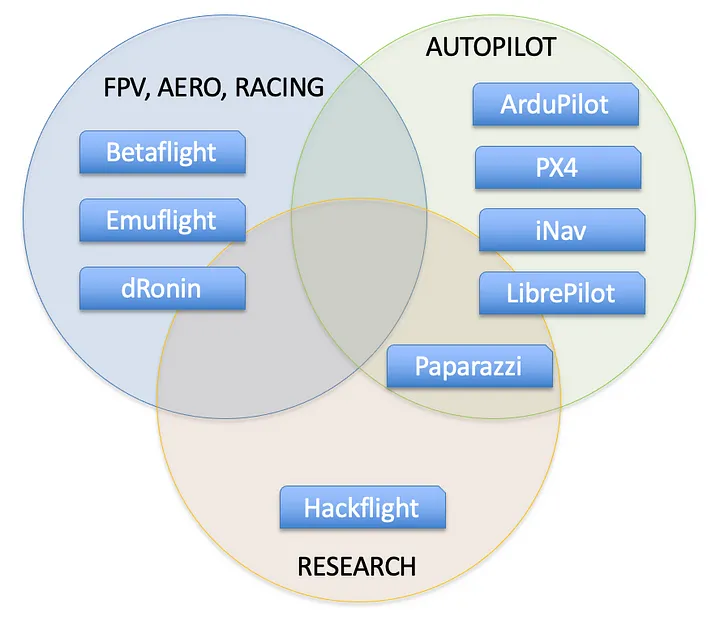
\includegraphics[width=0.6\textwidth]{opensource-autopilots.png}
    \caption[Categorización de software autopiloto de código abierto.]{Categorización de software autopiloto de código abierto.\footnotemark}
    \label{fig:opensource-autopilots}
\end{figure}
\footnotetext{\url{http://archive.today/2023.05.19-181849/https://reefwing.medium.com/a-review-of-open-source-flight-control-systems-2fe37239c9b6}}

\section{Planteamiento del problema}

\textbf{Los software controladores de RPAS mantenidos actualmente como ArduPilot o Pixhawk incluyen sistemas de autopiloto y vuelo asistido generalmente a base de algoritmos PID.} En algunos casos como con Pixhawk los detalles de implementación del controlador están documentados \cite{px4-control-diagram}, permitiendo que un usuario experimentado pueda \textbf{ajustar los parámetros en busca de un mejor desempeño.} \emph{Quizás se quiera lograr un vuelo más estable si se está pilotando manualmente \cite{betaflight-pid-tuning}, o en misiones autónomas reducir el consumo de las baterías, maximizar la distancia a recorrer o reducir el tiempo que una misión pueda tomar}. Otra manera de lograr estos objetivos \textbf{puede ser reemplazando por completo el algoritmo PID por controladores basados en modelos dinámicos como lo son LGR y LQR.} Si bien estos tipos de controlador han sido probados \cite{yt-lqr} los software autopiloto no ofrecen una arquitectura accesible que permita el prototipado rápido y la validación de estos sistemas. El prototipado rápido en este caso definido como el abrir acceso al código de los algoritmos para su modificación e iteración, donde se encuentren las entradas de los sensores y se genere la acción de control. La validación del sistema modificado sería el confirmar que en cierto contexto el algoritmo de control se pueda sintonizar a una aeronave y ejecutar planes de vuelo adecuadamente. Debido a lo experimental de una arquitectura así y lo costoso que puede ser una aeronave no tripulada se decide por su implementación en un ambiente simulado. Específicamente la verificación con X-Plane, donde el prototipado se realizaría con un autopiloto que maneje una aeronave en simulación y la validación tendría valor al lograrse la sintonización de aeronaves simuladas, pero desarrolladas por equipos profesionales donde el vuelo es comparable con la realidad.

\section{Objetivo}

Implementación de una arquitectura para validación de nuevos algoritmos de control en microcontroladores para aeronaves de ala fija por medio de técnica ``Hardware-in-the-Loop'' con X-Plane.

\subsection{Objetivos específicos}

\textbf{1.} Estudio de algoritmos de control y opciones de personalización disponibles para estos en los software de autopiloto actuales y selección de software autopiloto base.

\textbf{2.} Desarrollo de extensión de protocolo de comunicación de X-Plane para controladores autopiloto.

\textbf{3.} Implementación de distintos algoritmos de control a los ya implementados en el software y validación en simulador X-Plane como prototipo de arquitectura.

\textbf{4.} Establecer y documentar proceso sistemático para la implementación de algoritmos de control en la nueva arquitectura.

\section{Condiciones de diseño}

Al tratarse de un trabajo para el laboratorio de técnicas aeroespaciales, es de especial interés que la arquitectura sea accesible para alumnos y docentes en la facultad y el actual informe debe poder servir de documentación. Para estructurar la presentación del proyecto este se puede dividir en dos partes, el entorno de desarrollo que servirá como base para la investigación en X-Plane con un autopiloto, y el estudio de diseño de algoritmos de control.

\subsection{Entorno de desarrollo}

El entorno de desarrollo debe ser construido como una extensión del protocolo de comunicación con X-Plane establecido en el proyecto de ingeniería \cite{pia}, habilitando una interfaz a microcontroladores con software autopiloto donde X-Plane emule las funciones que haría una aeronave real. X-Plane debe proporcionar lecturas de sensores simulados y responder apropiadamente a entradas de control de radio lo cual es una técnica conocida como ``Hardware-in-the-Loop'' \cite{pil}. Esta técnica facilita que el trabajo realizado en simulación pueda ser aplicado en aeronaves reales, puesto que para el controlador autopiloto no existirá diferencia entre estar conectado a X-Plane o funcionando en una aeronave real. Los autopilotos además se conectan a un software de estación en tierra que habilita una interfaz gráfica que permite monitorear el vuelo y crear una ruta para la misión \cite{ardupilot-gs}, entre otras cosas. El diseñar la arquitectura alrededor de software como ArduPilot o PX4 permite aprovechar todas estas funciones existentes. Los sistemas de autopiloto cuentan con interfaces estandarizadas para conectar sensores y entradas de radiocontrol. Es imperativo seleccionar una base que cuente con estos estándares definidos para la posterior implementación de los sensores simulados y la entrada de radiocontrol. El autopiloto base debe ser uno de los que ya se tenga experiencia en el laboratorio como PX4 o ArduPilot.

\begin{figure}[h]
    \centering
    \includesvg{pil.svg}
    \caption{Técnica ``Hardware-in-the-Loop''.}
    \label{fig:pil}
\end{figure}

\subsection{Diseño de algoritmos de control}

La funcionalidad de habilitar la modificación de los algoritmos de control existentes o la implementación de uno nuevo debe incorporar el uso de lenguajes diseñados para ello, como Simulink, en el que se tenga acceso a las entradas como lecturas de los sensores y a generar acciones de control. Un algoritmo podrá ser validado en el software de simulación X-Plane como primera iteración, en este se podrá probar la interfaz entre el controlador de vuelo y X-Plane, la capacidad de sintonizar el algoritmo a aeronaves específicas y la realización de misiones autónomas. Esto será parte de un proceso sistemático con instrucciones con el objetivo final de que los algoritmos puedan ser probados en aeronaves reales. El procedimiento de diseño de controladores fomentará la experimentación con base en herramientas ya utilizadas en el laboratorio como lo son Simulink o Python. Con especial enfoque en aeronaves de ala fija.

\section{Metodología de trabajo}

\subsection{Selección de autopiloto base}

A partir de las condiciones de diseño establecidas se realizará una comparación entre las soluciones de autopiloto existentes. Además se investigarán trabajos ya realizados que hayan tenido objetivos similares a los de este proyecto, en especial el de modificar e implementar algoritmos de control puesto que en mi opinión es la parte más difícil.

\subsection{Extensión de protocolo}

Con el autopiloto base seleccionado, se debe proceder a replicar las interfaces de hardware estandarizadas para simular la experiencia de una aeronave real, donde X-Plane junto al protocolo de comunicación la emularan. Los datasheets de los sensores disponibles serán utilizados para replicar las señales que estos entregan al controlador de acuerdo a su capacidad o precisión. Se estudiaran los factores adversos que pudiesen ocurrir afectando la radiofrecuencia de control debido al clima o distancias para también hacer una estimación de ellos. Todo esto se implementará en el software inoFS \cite{inofs} en su programación. Para la interfaz de hardware se conectará a la Raspberry Pi Pico un bus de comunicación de acuerdo al estándar de autopiloto \cite{px4-bus}, sea uno proporcionado por el laboratorio o replicado con los insumos electrónicos que se deban comprar. Para que este objetivo pueda ser logrado no hace falta modificar el código del autopiloto, si los algoritmos PID logran funcionar con simulaciones de X-Plane es suficiente.

\subsection{Prototipo de implementación de nuevos algoritmos}

Ya sea a partir de esfuerzos previos realizados por la comunidad o el estudio del código fuente del autopiloto base se implementara otro sistema de control que se ejecute en el microcontrolador con el software de autopiloto. Al existir la extensión de protocolo probada con PID el funcionamiento del nuevo prototipo de controlador podrá ser verificado en X-Plane de la misma manera. El desarrollo del nuevo algoritmo será a partir de sistemas creados en Simulink y Python, donde el código final será exportado a C o C++ para su integración en el microcontrolador de autopiloto. El objetivo se considerará listo cuando se demuestre que el nuevo algoritmo logra cumplir tareas básicas como estabilización o el ajuste autónomo de las condiciones de vuelo a otras condiciones preestablecidas.

\subsection{Formulación de metodología para implementación de algoritmos}

Durante el desarrollo del prototipo probablemente se habrán intentado varias alternativas para lograr el funcionamiento adecuado, el último objetivo es preparar una metodología junto a documentación que defina el camino adecuado para la implementación de nuevos algoritmos en microcontroladores con software de autopiloto. Se reducirá el procedimiento a los pasos mínimos esenciales en documentación web del repositorio de inoFS, además de lo reportado en el informe de memoria de título. La metodología abarcará desde la creación de un algoritmo sencillo hasta su verificación en X-Plane.